\begin{enumerate}[label=\thesection.\arabic*.,ref=\thesection.\theenumi]
\numberwithin{equation}{enumi}
\item Plot the Bode magnitude and phase plots for the following system
\begin{align}
G\brak{s} &= \frac{Ks^2}{{\brak{1+0.2s}{\brak{1+0.02s}}}}
\label{eq:es17btech11002_system}
\end{align}
Also compute gain margin and phase margin .
\\
\solution Substituting $s=j\omega$ in   \eqref{eq:es17btech11002_system} 
\\
Initially assuming K =1
\begin{align}
G\brak{j\omega}&=\frac{\brak{j\omega}^2}{{\brak{1+0.2j\omega}}{\brak{1+0.02j\omega}}}
\end{align}
The corner frequencies are
\begin{align}
\omega{c1}=1/0.2 = 5rad/sec
\\
\omega{c2}=1/0.02 = 50rad/sec
\end{align}
\item Magnitude Plot Calculation.
\\
\solution
\begin{multline}
20log\abs{G\brak{j\omega}} = 20log\abs{\brak{j\omega}^2}-20log\abs{\brak{1+0.2j\omega}}\\\ -20log\abs{\brak{1+0.02j\omega}}
\end{multline}
The various values of G\brak{j\omega} are below TABLE  \ref{table:es17btech11002_1}, in the increasing order of their corner frequencies also slope contributed by each term and the change in slope at the corner frequency.
\begin{table}[!ht]
\centering
\input{./table/es17btech11002_1.tex}
\caption{Magnitude}
\label{table:es17btech11002_1}
\end{table}
\item Phase Angle Calculation
\\
\solution
\begin{align}
\phi = \angle{Gj\omega}= 180\degree-tan^{-1}\brak{0.2\omega}-tan^{-1}\brak{0.02\omega}
\end{align}
The phase angle of G\brak{j\omega} are calculated for various value of $\omega$ TABLE \ref{table:es17btech11002_2}.
\begin{table}[!ht]
\centering
\input{./table/es17btech11002_2.tex}
\caption{Phase}
\label{table:es17btech11002_2}
\end{table}
\\
The magnitude and phase plot are as follows: Fig\ref{fig:es17btech11002}
\begin{figure}[!h]
\centering
  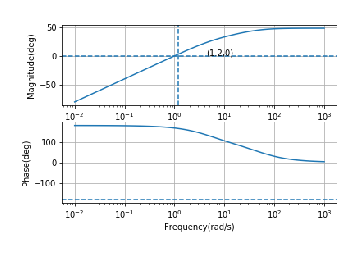
\includegraphics[width=\columnwidth]{./figs/es17btech11002.eps}
  \caption{Graphs}
  \label{fig:es17btech11002}
\end{figure}
\\
The python code to obtain the graphs:
\begin{lstlisting}
codes/es17btech11002.py
\end{lstlisting}

\item Calculation for K
\\
\solution 
The gain crossover frequency is 2rad/sec,
\\
At $\omega$ = 2, gain= 13db
\begin{align}
20log K= -13db
\\
Log K = -13/20
\implies
K= 0.65
\end{align}

\item Finding the Phase Margin \brak{PM} where $\omega_{gc}$ is frequency when gain = 1. This is known as phase margin(PM).
\\
\solution
\begin{align}
G\brak{j\omega}&=\frac{\brak{j\omega}^2}{{\brak{1+0.2j\omega}}{\brak{1+0.02j\omega}}}
\label{eq:es17btech11002_gain}
\end{align}
Solving \eqref{eq:es17btech11002_gain} or from Fig \ref{fig:es17btech11002} frequency at which gain = 1 ,is gain crossover frequency $\omega_{gc}$ .
\begin{align}
\omega_{gc} &=  1.2 \\
\implies
PM &=344.8
\end{align}
\item Find $-G(\j\omega)  $ db , where $\omega$ is frequency when phase = $-180\degree$ . This is known as  {\em gain margin} (GM)
\\
\solution From Fig \ref{fig:es17btech11002} ,we can say that phase  never crosses $-180\degree$ .
So , the gain margin is {\em infinite}.
Which means we can add any gain , and the equivalent closed loop system never goes unstable.
\end{enumerate}
